 \documentclass[main.tex]{subfiles}
 
\begin{document}

\chapter{stellar model}

\section{structure equations} 

\subsection{Dynamical stability}

Una regione stellare \'e convettivamente stabile se una perturbazione di densit\'a infinitesima non cresce ad ampiezza finita.
\begin{align*}
&\rho\PtwoDy{t}{(\Delta r)}=-g\Delta\rho\\
&=-g[\Dcvar{\TDy{r}{\rho}}{e}-\Dcvar{\TDy{r}{\rho}}{amb}]\Delta r
\end{align*}

La forza di Archimede ha verso opposta alla perturbazione se
\begin{equation*}
[\Dcvar{\TDy{r}{\rho}}{e}-\Dcvar{\TDy{r}{\rho}}{amb}]>0
\end{equation*}

\begin{figure}[!ht]
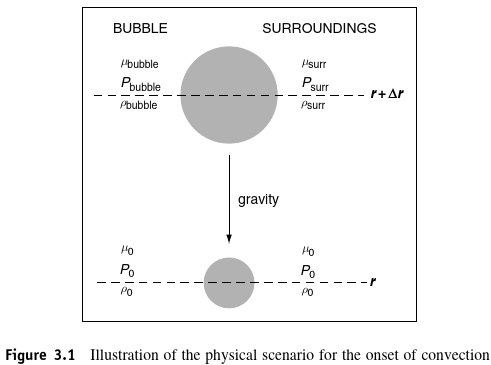
\includegraphics[trim={0cm 0cm 1cm 0cm},clip, keepaspectratio,width=0.99\textwidth]{convectivestability}\label{fig:convectivestability}
\end{figure}

\begin{itemize}
    \item Rayleigh-Taylor instability: $\TDy{r}{\ln{(\mu)}}>0$
    \item $\nrad>\nad-\frac{\xi_{\mu}}{\xi_T}\TDly{(P)}{(\mu)}$
\end{itemize}
		
\subsection{Gradiente ambientale nelle regioni convettive}



\chapter{evolution of stars}

\subsection{Massa minima innesco fusione H}

Temperatura minima per innesco idrogeno: $T_{min}\approx\SI{1.5e6}{\kelvin}$
\begin{align*}
&P_c=K_{NR}n_e\expy{5/3}+n_ikT_c=K_{NR}\frac{\rho_c}{m_H}]\expy{5/3}+\frac{\rho_c}{m_H}kT_c\\
&kT_c=A\rho_c\expy{1/3}-B\rho_c\expy{2/3}\\
&kT_{c,max}\propto G^2\frac{m_H\expy{8/3}}{K_{NR}}M\expy{4/3}
\end{align*}

\subsection{Massa massima}

\begin{align*}
&P=P_i+P_e+P_R=\frac{\rho_c}{\mu m_H}kT_c+\frac{1}{3}aT_c^4\\
&P_g=\beta P_c\quad P_R=(1-\beta)P_c
\end{align*}

\subsection{Struttura stellare approssimata}

\begin{itemize}
\item \keyword{Approssimazione zero per $M_r(0)$ e $M_r(R)$}:
Al centro della stella $\TDy{r}{P}=-\frac{GM_r}{r^2}\rho\approx-\frac{4\pi}{3}r^3\rho_c\frac{G}{r^2}\rho_c\approx-\frac{4\pi}{3}rG\rho_c^2$, vicino alla superficie $\TDy{r}{P}\approx-G\frac{M\rho}{r^2}$: se la composizione chimica \'e costante
\begin{align*}
&\TDy{r}{P}\approx-\frac{4\pi}{3}G\rho_c^2r\exp{-r^2/a^2}\\
&P(r)\approx-\frac{2\pi}{3}G\rho_c^2a^2[\exp{-r^2/a^2}-\exp{-R^2/a^2}]
\end{align*}

$4\pi\rho r^2dr=dm$ ci permette di riscrivere equilibrio idrostatico $GM_rdM_r=-4\pi r^4dP$:
\begin{align*}
&\frac{1}{2}GM_r^2=-4\pi\int_0^rr'^4\TDy{r}{P}\,dr\\
&M_r=\frac{4\pi a^3}{3}\rho_c\Phi(x)\quad x=r/a\\
&\Phi(x)=6\int_0^xx'^5\exp{-x'^2}\,dx'\approx x^6-3/4x^8+3/10x\expy{10}+...
\end{align*}
per alta $\rho_x$ $a\ll R$ ...:
\begin{align*}
&M\approx M_r=\frac{4\pi\rho_ca^3}{3}\Phi(\frac{R}{a})\approx\frac{4\pi\rho_ca^3}{3}\sqrt{6}\\
&P_c\approx\frac{2\pi}{3}G\rho_c^2a^2\approx[\frac{\pi}{36}]GM\expy{2/3}\rho_c\expy{4/3}
\end{align*}

\item Politropa $n=3/2$: $P_c\propto M\expy{2/3}\rho_c\expy{4/3}$

\item Politropa $n=3$: $P_c\propto M\expy{2/3}\rho_c\expy{4/3}$

\end{itemize}

\section{Evolution scaling}

\begin{itemize}
    \item \xaumenta{M}, \xdiminuisce{\tau}
    \item \xdiminuisce{M}, \xaumenta{\rho_c}, \xdiminuisce{T_c}
    \item \xaumenta{Z}, \xdiminuisce{L}, \xdiminuisce{T_e}, \xaumenta{\tau}
    \item \xaumenta{Y}, \xaumenta{L}, \xaumenta{T_e}, \xdiminuisce{\tau}
    \item Opacit\'a in funzione di Y: \xaumenta{Y}, \xdiminuisce{\kappa} 
\end{itemize}

\subsection{Low mass star}

tempi evolutivi in HRD


\section{From proto-star to Pre-MS}

\begin{itemize}
\item Isothermal collapse of MC ($t_{cool}\ll t_{ff}$, $P\propto\rho$). MC build up as gas flow into arm's potential well. massa di Jeans $M_J\propto\expy{3/2}\rho\expy{-1/2}$. $M_j$ diminuisce all'aumentare di densit\'a: frammentazione
\item Virial theorem.

\adjm{\rho\TDy{t}{\vec{u}}=-\nabla P-\rho\nabla\phi+\frac{1}{c}\vecp{j}{B}}

\adjm{\rho\TDy{t}{\vec{u}}=-\nabla P-\rho\nabla\phi+\frac{1}{4\pi}(\scap{B}{\nabla})\vec{B}-\frac{1}{8\pi}\nabla|B|^2}

\adjm{\frac{1}{2}\PtwoDy{t}{I}=2T+2U+W+M}

\adjm{I=\int \rho|r|^2\,d^3x,\ T=\frac{1}{2}\int\rho|\vec{u}|^2\,d^3x,\ U=\frac{3}{2}\int nKT\,d^3x=\frac{3}{2}\int P\,d^3x}

\adjm{W=\frac{1}{2}\int\rho\phi\,d^3x\ M=\frac{1}{8\pi}\int|B|^2\,d^3x}

No evidence for collapse of giant complexes: $2T+2U+W+M$.

\adjm{\frac{T}{|W|}\approx\frac{1}{2};\Delta V^2\invers{(\frac{GM^2}{R})}}

\adjm{=0.5(\frac{\Delta V}{\SI{4}{\kilo\meter\per\second}})^2(\frac{M}{10^5\msun{}})\expy{-1}(\frac{R}{\SI{25}{\parsec}})}

\adjm{\Delta V\approx\sqrt{\frac{GM}{R}}=V_{vir},\ t_{ff}\approx\sqrt{\frac{R^3}{GM}}}

Small clumps moving moving in gravitational field of whole ensamble.
\item Denser regions with point IR source. (Fase adiabatica $P\propto\rho\expy{\gamma}$, $T\propto\rho\expy{2/3}$ per mono-ideal gas) Inner region of collapsing cloud becomes denser/optically thicker (first core formation $\tau\approx\SI{1.5e7}{\year}$): role of ambipolar diffusion. Typical mass $M_*=\num{e-2}\msun{}$, $R_*=\SI{5}{\astronomicalunit}$, $\rho\approx\SI{e-10}{\gram\per\cubic\cm}$. Energy radiated by denser core is absorbed by free-falling gas and re-emitted in IR
\item The first core of molecular hydrogen collapse as soon as T is raised enough to begins molecular dissociation (for $T>2000K$ we have collisional diss)
\begin{align*}
&0=-\frac{1}{2}\frac{GM_*^2}{R_*}+\Delta E_{int}+L_{rad}t\\
&L_{rad}\approx L_{acc}=\frac{\dot{M}GM_*}{R_*}\\
&\Delta E_{int}=\frac{XM_*}{m_H}[\frac{\Delta E_{dis}(H)}{2}+\Delta E_{ion}(H)]+\frac{YM_*\Delta E_{ion}(He)}{4m_H}
\end{align*}
\item Birthline
\begin{align*}
&\tau_{KH}=\frac{GM_*^2}{R_*L_*}\propto L_*\expy{-3/2}\\
&\TDy{t}{R_*}\propto-\frac{R_*}{t_{KH}}\\
&L_*=4\pi\sigma T_*^4R_*^2\\
&\TDy{t}{L_*}\propto-\frac{L_*}{\tau_{KH}}
&T_*\approx\const{}
\end{align*}
The most luminous therefore youngest object reflect its nature of accreting object within collapsing dense core: surface temperature and luminosity are set by infall (\numrange{e-5}{e-6}$\msun/yr$) dynamics (expected to change when infall end), radius by internal structure and is the same for protostar and pre-MS star; the birthline is the locus of pre-MS star with protostellar radii. At $M_*=8\msun$ the birthline intercept the ZAMS
\item Slower accretion give radius more time to shrink but D-burning thermostat limit that. D ignition: $^2H+^1H\to^3He+\gamma(\SI{5.5}{\mega\ev})$.
\item ''position'' of Hayashi track: \xaumenta{Y}, \xaumenta{T_e}; \xaumenta{Z}, \xdiminuisce{T_e}; \xdiminuisce{M}, \xdiminuisce{T_e}
\item formation of radiative core caused by \xdiminuisce{R}, \xdiminuisce{L}, \xdiminuisce{\nabla_{rad}} ($L\propto R^2$); parallelamente \xdiminuisce{R}, \xaumenta{T}, \xdiminuisce{\exv{\kappa}} ($\kappa_{kr}\propto$), \xdiminuisce{\nrad{}}, \xaumenta{T_e}
(stahler palla fig 16.8)
\end{itemize}

\subsection{Pre-MS star model}
Structure equation:
\begin{align*}
&\PDy{M_r}{r}=\frac{1}{4\pi r^2\rho}\\
&\PDy{M_r}{P}=-\frac{GM_r}{4\pi r^4}\\
&\PDy{M_r}{L_{int}}=\epsilon-T\PDy{t}{s}
\end{align*}
fourth equation in radiative/convective zones
\begin{align*}
&T^3\PDy{M_r}{T}=-\frac{3\kappa L_{int}}{256\pi^2\sigma r^4}\\
&\PDy{M_r}{s}
\end{align*}
HE integrated from phot to inf
\adjm{P_{phot}=\frac{GM_*}{R_*^2}\int_{R_*}^{\infty}\rho\,dr\approx\frac{GM_*}{R_*^2\kappa_{phot}}\int_{R_*}^{\infty}\rho\kappa\,dr=\frac{GM_*\Delta\tau}{R_*^2\kappa_{phot}}}
(adim eqs:
\adjm{x=\frac{r}{R},\ q=\frac{M_r}{M},\ t=\frac{T}{T_0},\ p=\frac{P}{P_0},\ T_0=\frac{\mu GMm_H}{Rk},\ P_0=\frac{GM^2}{4\pi R^4}}
Continuity: $\TDy{x}{q}=\frac{p}{t}x^2$, HE: $\TDy{x}{p}=-\frac{p}{t}\frac{q}{x^2}$, $\nad$ for fully convective star: $P=CT\expy{5/2}\to p=Et\expy{2.5}$ (C determines the adiabat).
HayT is vertical $\TDly{T_e}{L}>10$, mild mass deps $\TDly{M}{T_e}\approx0.2$. Realistically: surface condition+super-adibat layer.
)

As T increses due to contraction (V.T.)a central radiative core is formed: when a sizeble radiative core formed path toward higher $T_e$ is almost horizontal.
At temperature \SIrange{1e6}{2.5e6}{\kelvin} D/Li(Be/B) are burnt by proton capture (Li/D depletion at surface for fully convective star).
In general larger masses have lower Li depletion, given mass increases increasing Z: \xaumenta{M}(or \xdiminuisce{Z}) lower convective zone but also earlier retreat from center (fig 16.10)


\section{Sequenza principale}

\section{From H central exhaustion to He central ignition: overall contraction/TO to TRGB}

\subsection{Low mass stars ($M_{cSC}\approx0.1\msun$)}

\begin{itemize}
\item As H exhausts in center $T_M$ moves outward: at TO $90\%$ of H-burning in thick shell of $0.2\msun$: H-burning shell becomes thinner and thinner as CNO is strongly T-dep and as H-depleted inside and T drops in envelope.
\end{itemize} 

\end{document}